\documentclass[final]{beamer}

% ---------------------------------------------------------------------------
% Quantathon CR 2026 -- Challenge 3
% Poster (A0 vertical): Fermi-Hubbard en escalera 3x2 -- ED vs. Trotter vs. VQE
% Misma paleta que las presentaciones. Compilar desde Informe_tecnico/:
%   pdflatex poster_fermi_hubbard.tex
% Las figuras se leen de ../fermi_hubbard_*.png (generadas por el notebook a 300 dpi).
% Acompana a presentacion_fermi_hubbard_charla.tex (charla de 10 min).
% ---------------------------------------------------------------------------

\usepackage[orientation=portrait,size=a0,scale=1.4]{beamerposter}
\usepackage[utf8]{inputenc}
\usepackage[T1]{fontenc}
\usepackage{textcomp}
\usepackage{amsmath,amssymb}
\usepackage{booktabs}
\usepackage{graphicx}
\usepackage{tikz}
\usetikzlibrary{arrows.meta,positioning,calc}

\definecolor{qDeep}{RGB}{35,32,90}
\definecolor{qMid}{RGB}{75,55,160}
\definecolor{qAccent}{RGB}{0,150,170}
\definecolor{qWarn}{RGB}{190,60,50}
\definecolor{qGray}{RGB}{90,90,95}

\setbeamertemplate{navigation symbols}{}
\setbeamercolor{structure}{fg=qMid}
\setbeamercolor{block title}{fg=white,bg=qMid}
\setbeamercolor{block body}{bg=qMid!6}
\setbeamercolor{block title alerted}{fg=white,bg=qWarn}
\setbeamercolor{block body alerted}{bg=qWarn!7}
\setbeamercolor{block title example}{fg=white,bg=qAccent}
\setbeamercolor{block body example}{bg=qAccent!8}
\setbeamercolor{item}{fg=qAccent}
\setbeamertemplate{block begin}{\vskip0.6em
  \begin{beamercolorbox}[wd=\linewidth,sep=0.5em,leftskip=0.3em]{block title}%
    \usebeamerfont*{block title}\strut\insertblocktitle\strut\end{beamercolorbox}%
  \vskip-0.1em
  \begin{beamercolorbox}[wd=\linewidth,sep=0.6em,leftskip=0.3em,rightskip=0.3em]{block body}%
    \usebeamerfont{block body}}
\setbeamertemplate{block end}{\end{beamercolorbox}\vskip0.3em}
\setbeamertemplate{block alerted begin}{\vskip0.6em
  \begin{beamercolorbox}[wd=\linewidth,sep=0.5em,leftskip=0.3em]{block title alerted}%
    \usebeamerfont*{block title}\strut\insertblocktitle\strut\end{beamercolorbox}%
  \vskip-0.1em
  \begin{beamercolorbox}[wd=\linewidth,sep=0.6em,leftskip=0.3em,rightskip=0.3em]{block body alerted}}
\setbeamertemplate{block alerted end}{\end{beamercolorbox}\vskip0.3em}
\setbeamertemplate{block example begin}{\vskip0.6em
  \begin{beamercolorbox}[wd=\linewidth,sep=0.5em,leftskip=0.3em]{block title example}%
    \usebeamerfont*{block title}\strut\insertblocktitle\strut\end{beamercolorbox}%
  \vskip-0.1em
  \begin{beamercolorbox}[wd=\linewidth,sep=0.6em,leftskip=0.3em,rightskip=0.3em]{block body example}}
\setbeamertemplate{block example end}{\end{beamercolorbox}\vskip0.3em}
\setbeamerfont{block title}{size=\large,series=\bfseries}
\setbeamertemplate{itemize items}{\textbullet}

\newcommand{\good}[1]{\textcolor{qAccent}{\textbf{#1}}}
\newcommand{\warn}[1]{\textcolor{qWarn}{\textbf{#1}}}
% Mensaje clave al pie de cada bloque
\newcommand{\clave}[1]{\vspace{0.4em}\par\noindent\colorbox{qDeep}{\parbox{\dimexpr\linewidth-2\fboxsep}{\color{white}\textbf{#1}}}}

\begin{document}
\begin{frame}[t]

% =========================== ENCABEZADO ===================================
\begin{tikzpicture}[remember picture,overlay]
  \fill[qDeep] (current page.north west) rectangle ([yshift=-10cm]current page.north east);
  \fill[qAccent] ([yshift=-10cm]current page.north west) rectangle ([yshift=-10.5cm]current page.north east);
  \node[text=white,align=center,text width=0.95\paperwidth] at ([yshift=-5cm]current page.north) {
    {\fontsize{80}{96}\selectfont\bfseries Modelo de Fermi-Hubbard en una escalera 3\texttimes2\par}
    \vspace{0.8cm}
    {\Huge ¿Qué tan lejos llegan los métodos cuánticos frente a la solución exacta?\par}
    \vspace{0.8cm}
    {\Large Luis Corado \quad·\quad Carné 201903168 \quad·\quad Quantathon CR 2026 -- QWorld Hackathon, Challenge 3\par}
  };
\end{tikzpicture}
\vspace{10.2cm}

% Tablas un poco mas aireadas en todo el poster
\renewcommand{\arraystretch}{1.25}

% =========================== FILA 1 =======================================
\begin{columns}[T]
\begin{column}{0.02\paperwidth}\end{column}

\begin{column}{0.30\paperwidth}
  \begin{block}{1 · Modelo y métodos}
    \[
      H = -t\!\!\sum_{\langle ij\rangle,\sigma}\!\!\left(c^\dagger_{i\sigma}c_{j\sigma}+\text{h.c.}\right)
          + U\sum_i n_{i\uparrow}n_{i\downarrow} - \mu\!\sum_{i\sigma} n_{i\sigma}
    \]
    \centering
    \begin{tikzpicture}[scale=3.4,
        site/.style={circle,fill=qMid,text=white,minimum size=2cm,inner sep=0pt,font=\Large\bfseries}]
      \foreach \x in {0,1,2} {
        \node[site] (a\x) at (\x,0) {\the\numexpr\x\relax};
        \node[site] (b\x) at (\x,1) {\the\numexpr\x+3\relax};
        \draw[qAccent,line width=5pt] (a\x) -- (b\x);
      }
      \draw[qDeep,line width=5pt] (a0)--(a1)--(a2); \draw[qDeep,line width=5pt] (b0)--(b1)--(b2);
      \draw[qDeep,line width=5pt,dashed] (a2) to[bend left=40] (a0);
      \draw[qDeep,line width=5pt,dashed] (b2) to[bend right=40] (b0);
      \node[font=\normalsize,qGray] at (1,-0.7) {pierna periódica};
      \node[font=\normalsize,qAccent,rotate=90] at (-0.5,0.5) {peldaño};
    \end{tikzpicture}

    \vspace{0.4em}
    \begin{tabular}{@{}lcc@{}}
      \toprule
       & \textcolor{qGray}{plan $4{\times}2$} & \textbf{usado $3{\times}2$} \\
      \midrule
      Sitios / qubits & 8 / 16 & \textbf{6 / 12} \\
      Capas de Trotter & 7 & \textbf{9} \\
      $E_{\text{VQE}}/E_{\text{exacto}}$, $U{=}0$ & \warn{$-5.3/-12$} & \good{$-7.0/-8$} \\
      \bottomrule
    \end{tabular}

    \vspace{1em}
    \begin{tabular}{@{}lll@{}}
      \toprule
      \textbf{Método} & \textbf{Herramienta} & \textbf{Responde} \\
      \midrule
      ED & numpy / scipy & referencia exacta \\
      Trotter & Qiskit Aer & dinámica \\
      VQE & Qiskit & estado base \\
      \bottomrule
    \end{tabular}
    \clave{Llenado medio, $t=1$, barrido en $U/t$.}
  \end{block}
\end{column}

\begin{column}{0.02\paperwidth}\end{column}

\begin{column}{0.62\paperwidth}
  \begin{block}{2 · Diagonalización exacta: el crossover}
    \centering
    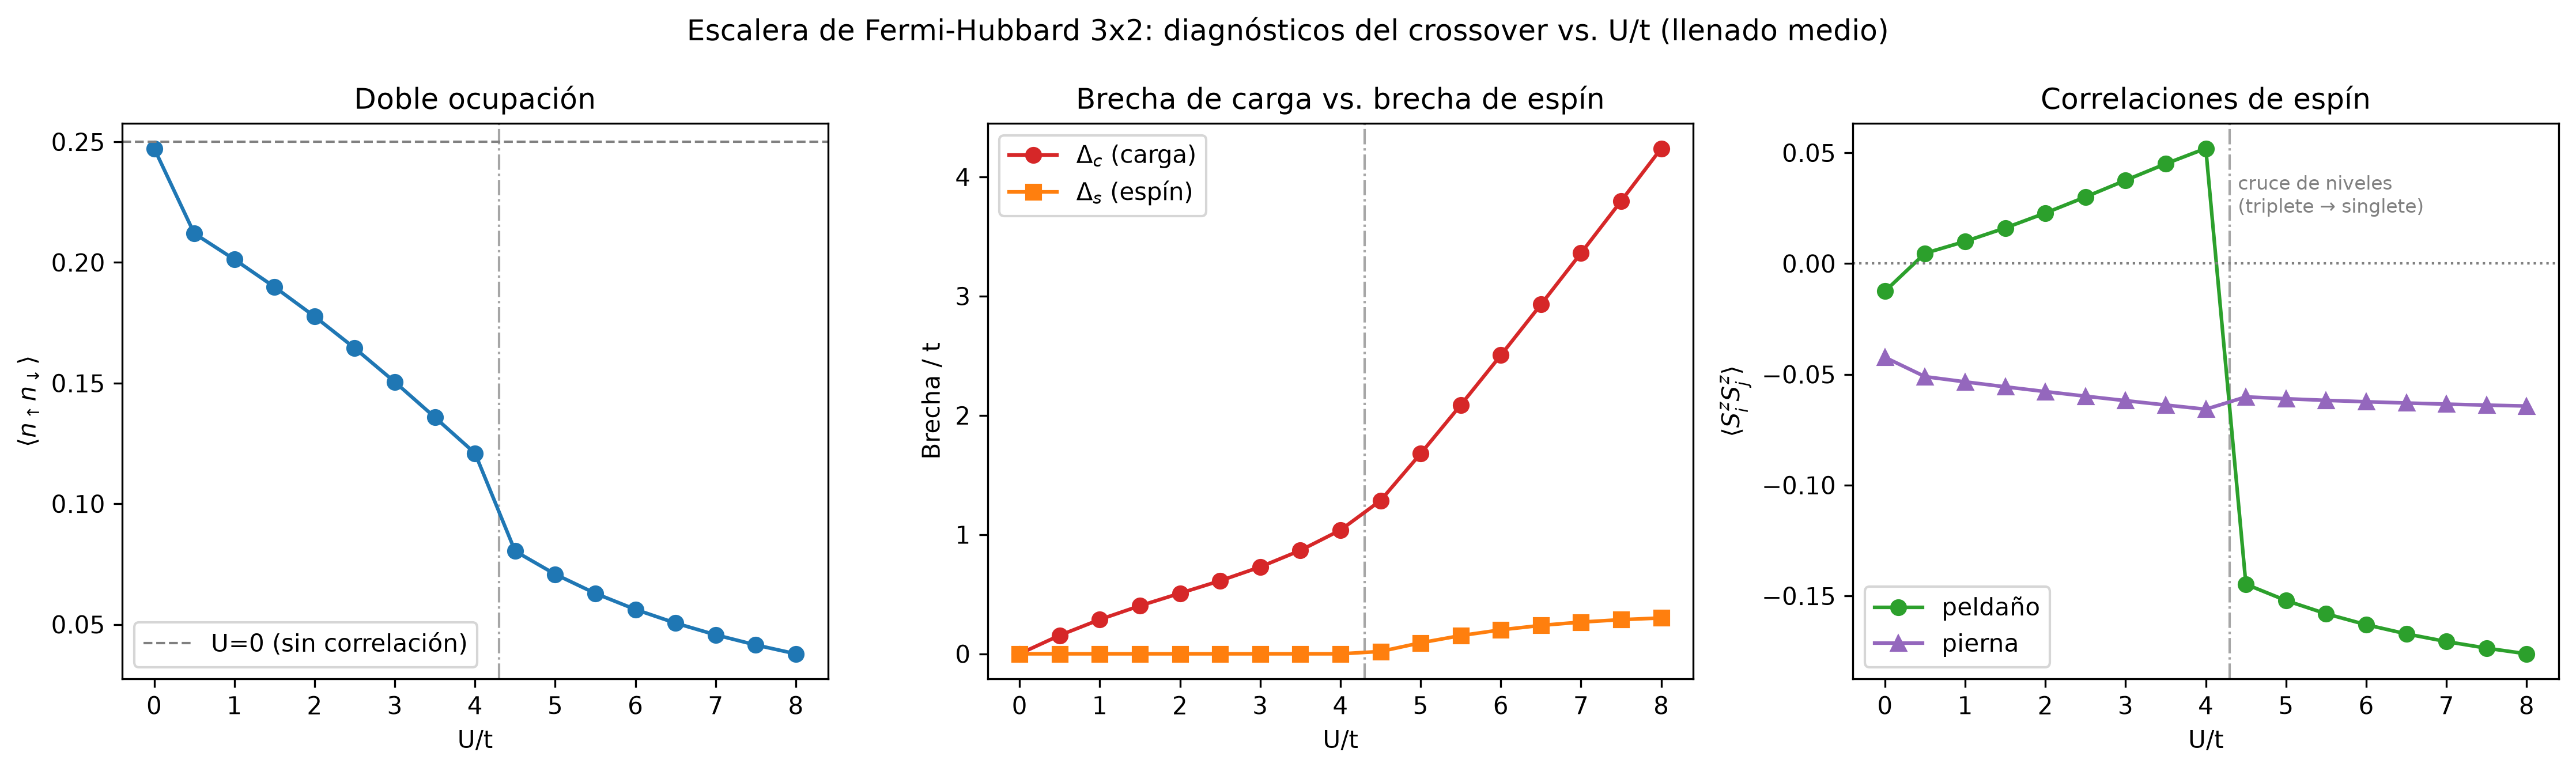
\includegraphics[width=\linewidth]{../fermi_hubbard_2d_phase_diagram.png}

    \vspace{0.6em}
    {\large
    \begin{tabular}{@{}lccccc@{}}
      \toprule
      $U/t$ & 0 & 2 & 4 & 5 & 8 \\
      \midrule
      Doble ocupación $D$ & 0.25 & 0.178 & 0.121 & 0.071 & 0.038 \\
      Brecha de carga $\Delta_c$ & 0 & 0.51 & 1.04 & 1.68 & 4.24 \\
      Brecha de espín $\Delta_s$ & 0 & 0 & 0 & \good{0.09} & \good{0.30} \\
      Correlación de peldaño & $-0.01$ & $+0.02$ & $+0.05$ & \good{$-0.15$} & \good{$-0.18$} \\
      \midrule
      Estado base & \multicolumn{3}{c}{\warn{triplete}} & \multicolumn{2}{c}{\good{singlete}} \\
      \bottomrule
    \end{tabular}}
    \clave{Crossover (no transición): $\Delta_c$ crece con $U$. Cruce de niveles de
      tamaño finito en $U/t\approx4.3$.}
  \end{block}
\end{column}

\begin{column}{0.02\paperwidth}\end{column}
\end{columns}

% =========================== FILA 2: TROTTER ==============================
\vfill
\begin{columns}[T]
\begin{column}{0.02\paperwidth}\end{column}
\begin{column}{0.96\paperwidth}
  \begin{exampleblock}{3 · Evolución de Trotter: decaimiento de doblones}
    \centering
    {\large Estado inicial: pierna $y{=}0$ llena, $y{=}1$ vacía \;\;·\;\; $D(0)=0.5$ \;\;·\;\;
      $T=5$ \;\;·\;\; 50 pasos \;\;·\;\; 2000 shots}

    \vspace{0.6em}
    \begin{columns}[T]
      \begin{column}{0.49\linewidth}
        \centering {\large\textbf{$U/t=1$: los doblones decaen}}\\[0.3em]
        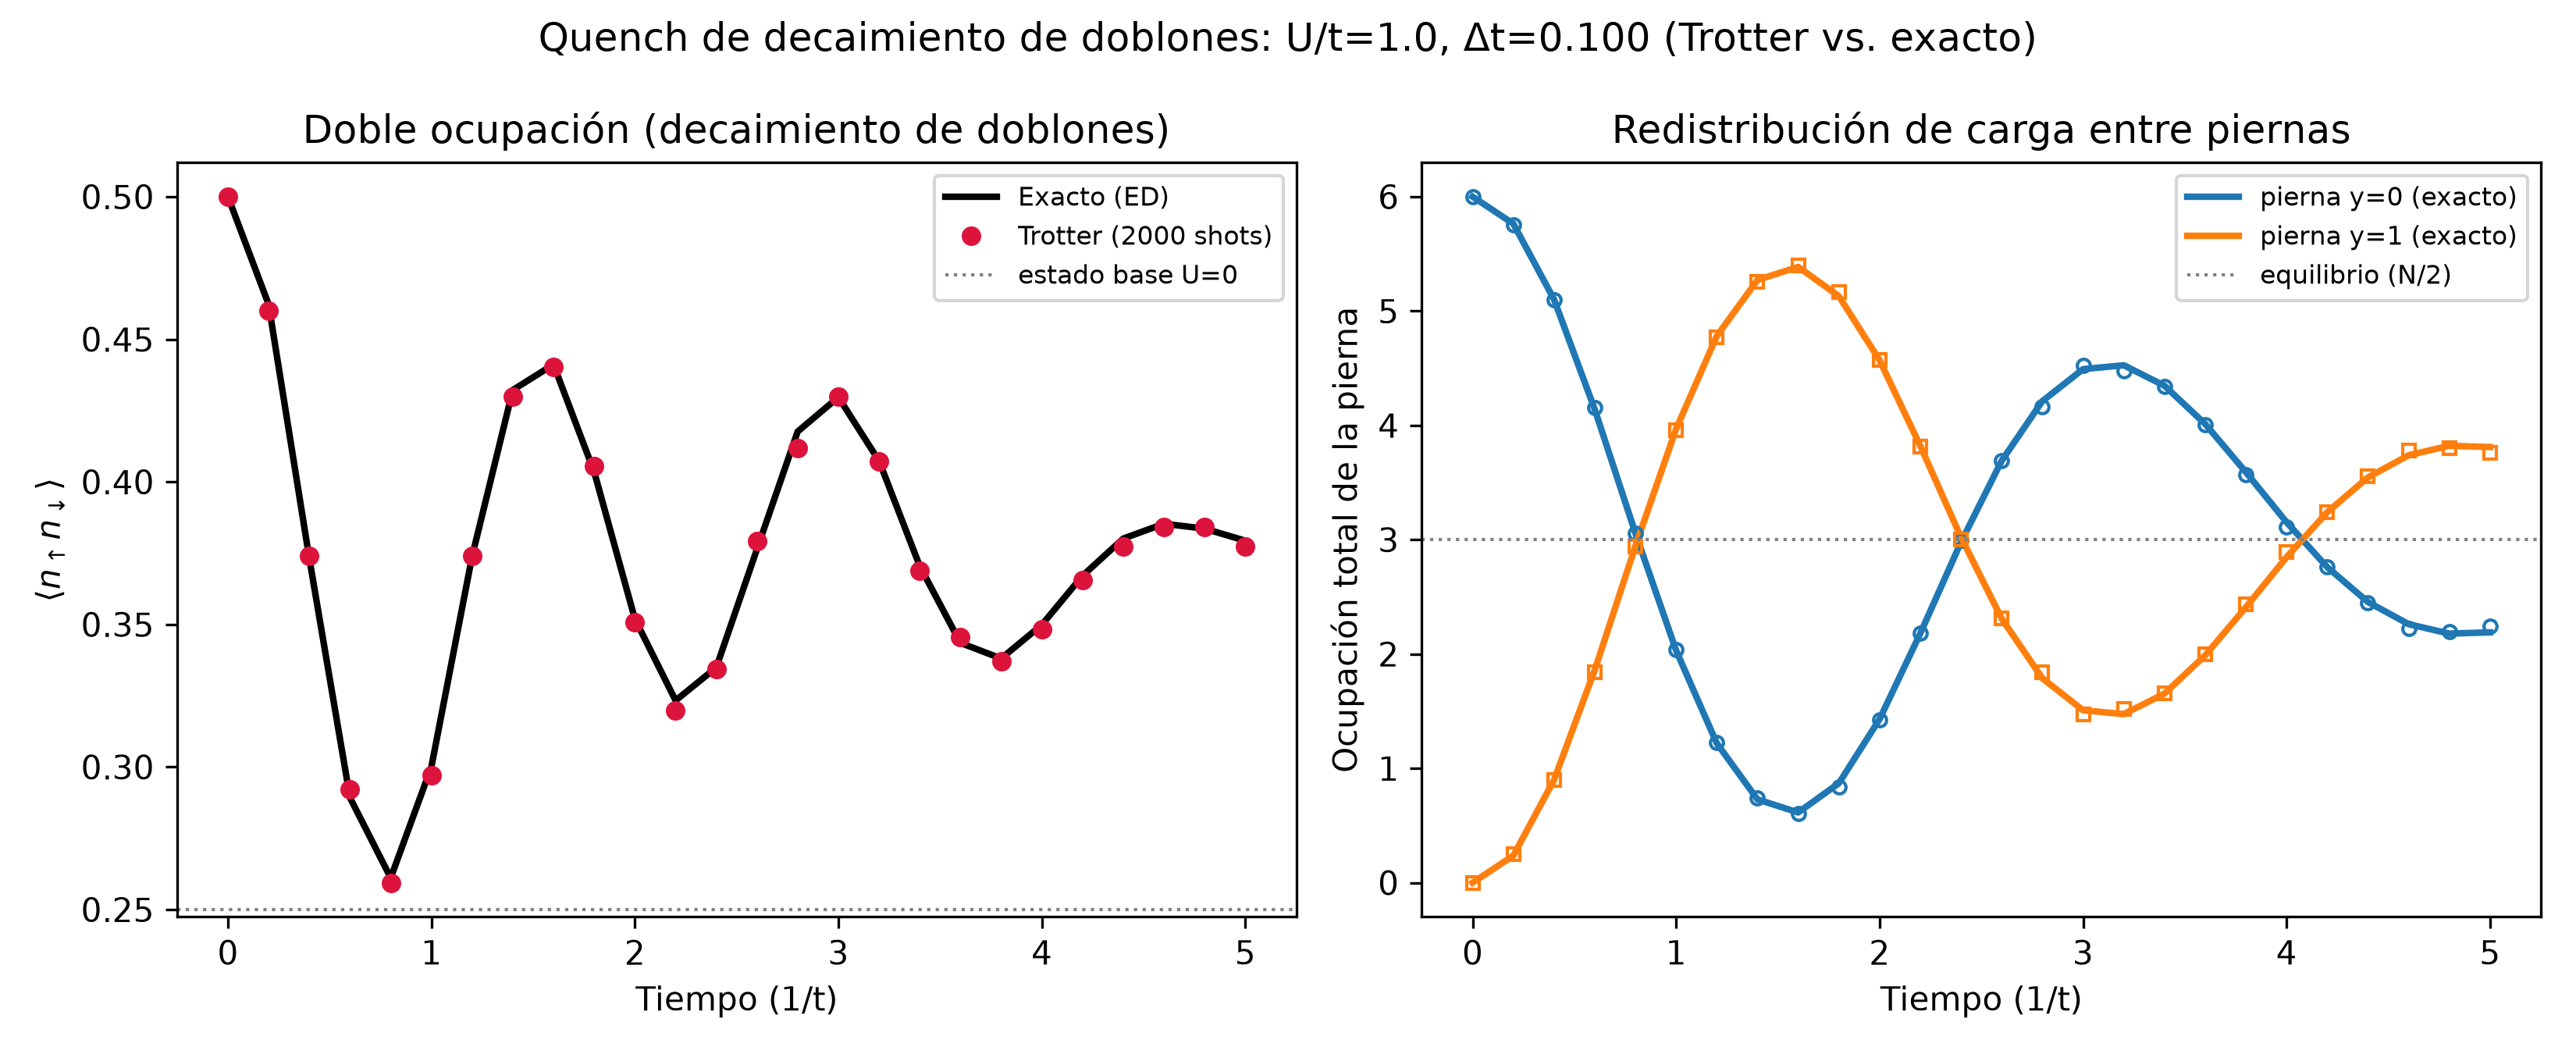
\includegraphics[width=\linewidth]{../fermi_hubbard_quench_U1.0_trotter_vs_exact.png}
      \end{column}
      \begin{column}{0.49\linewidth}
        \centering {\large\textbf{$U/t=8$: decaimiento suprimido}}\\[0.3em]
        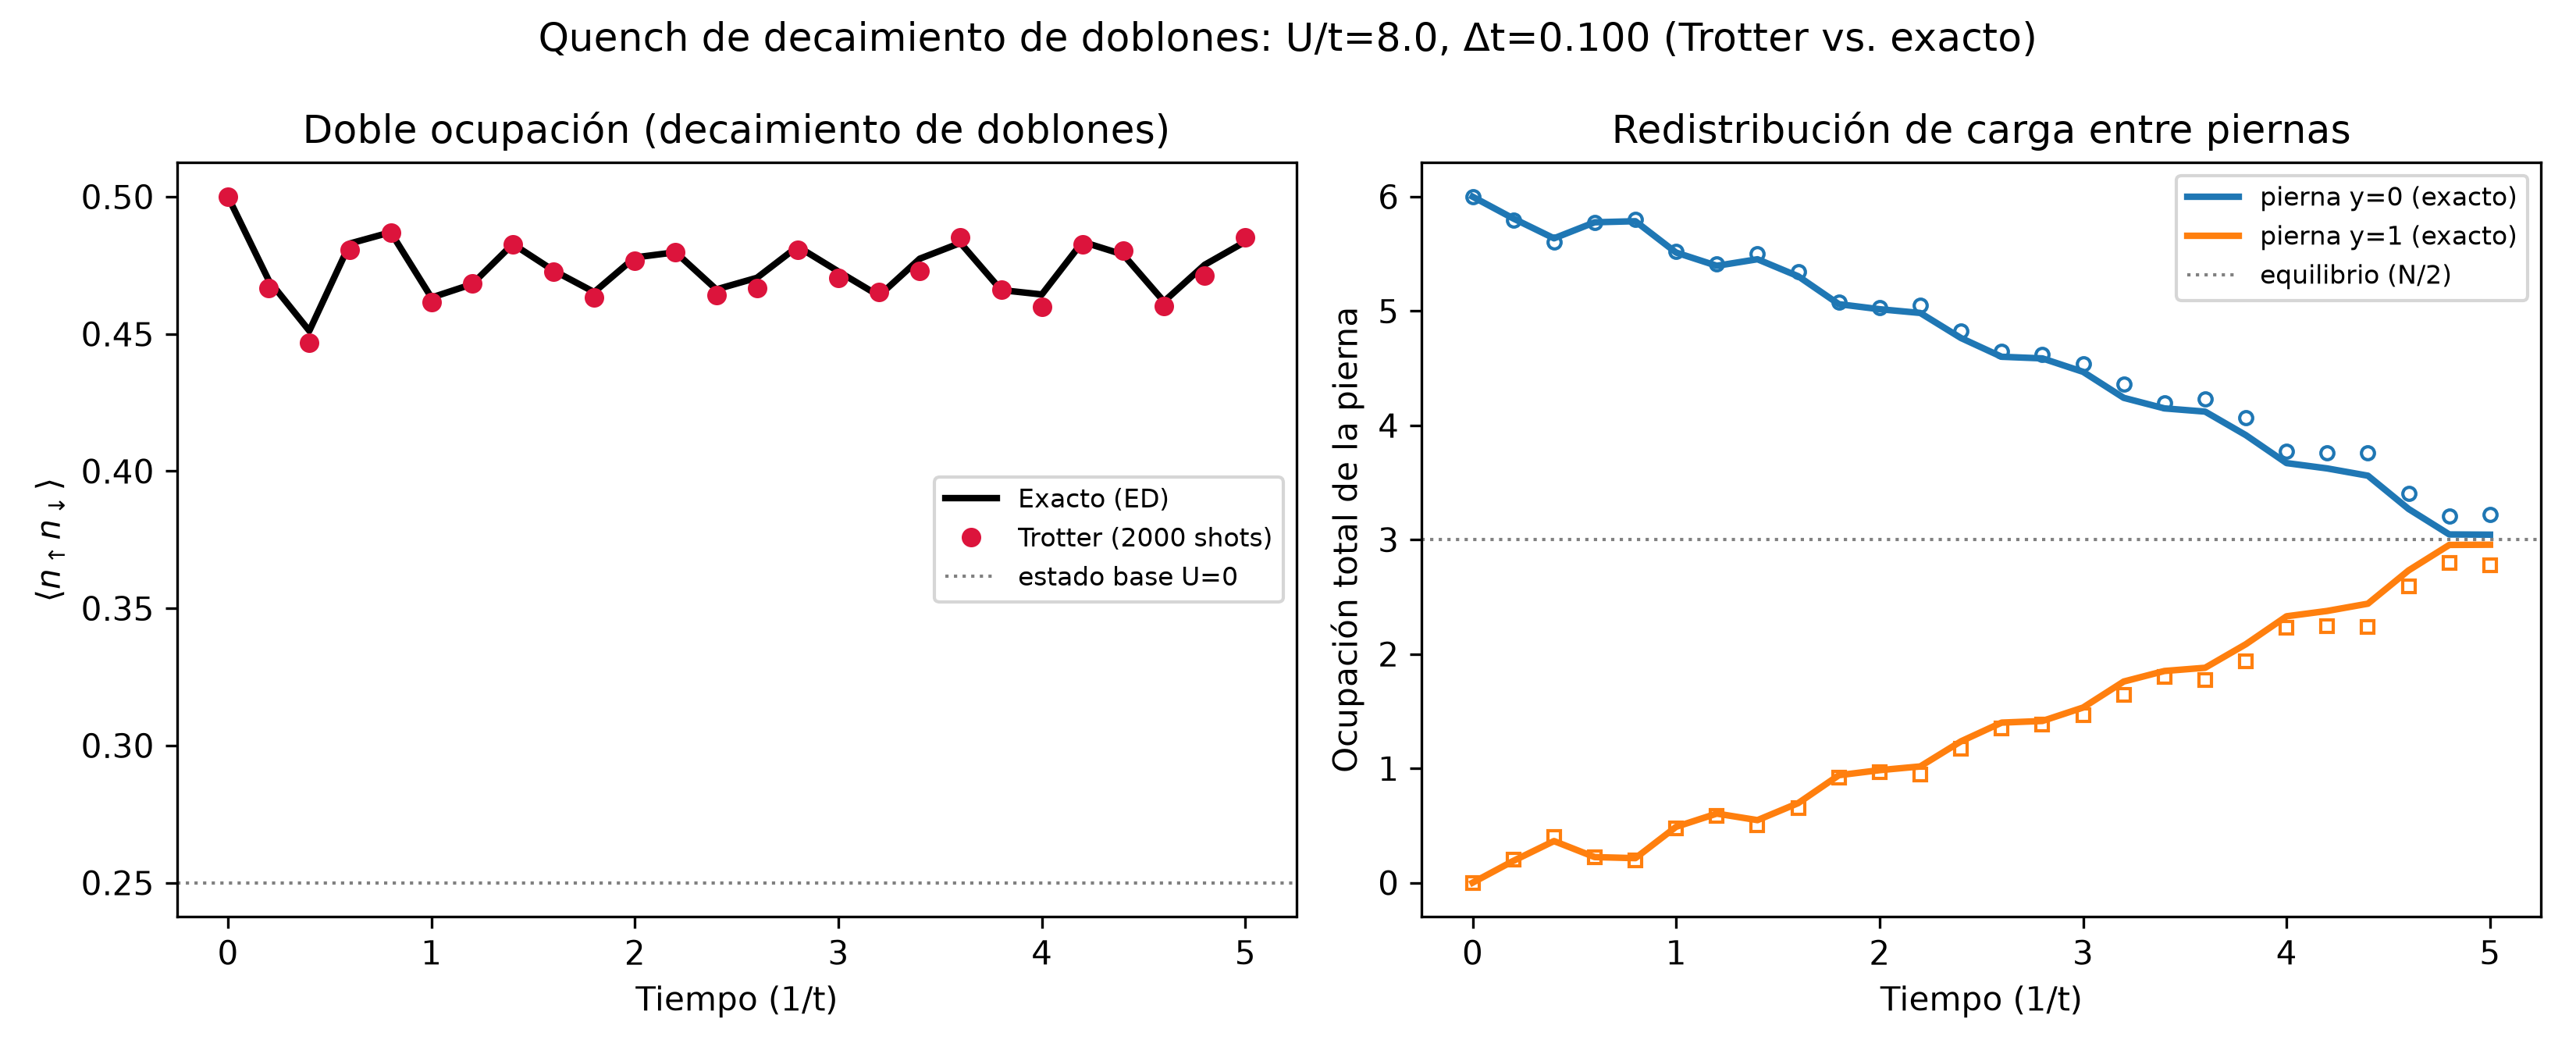
\includegraphics[width=\linewidth]{../fermi_hubbard_quench_U8.0_trotter_vs_exact.png}
      \end{column}
    \end{columns}
    \clave{Trotter = exacto dentro del ruido de shots ($|\Delta D|\sim$0.001--0.005).
      A $U\gg t$ los doblones no decaen.}
  \end{exampleblock}
\end{column}
\begin{column}{0.02\paperwidth}\end{column}
\end{columns}

% =========================== FILA 3: C y D ================================
\vfill
\begin{columns}[T]
\begin{column}{0.02\paperwidth}\end{column}

\begin{column}{0.30\paperwidth}
  \begin{block}{4 · Error de Trotter ($U/t=4$)}
    \centering
    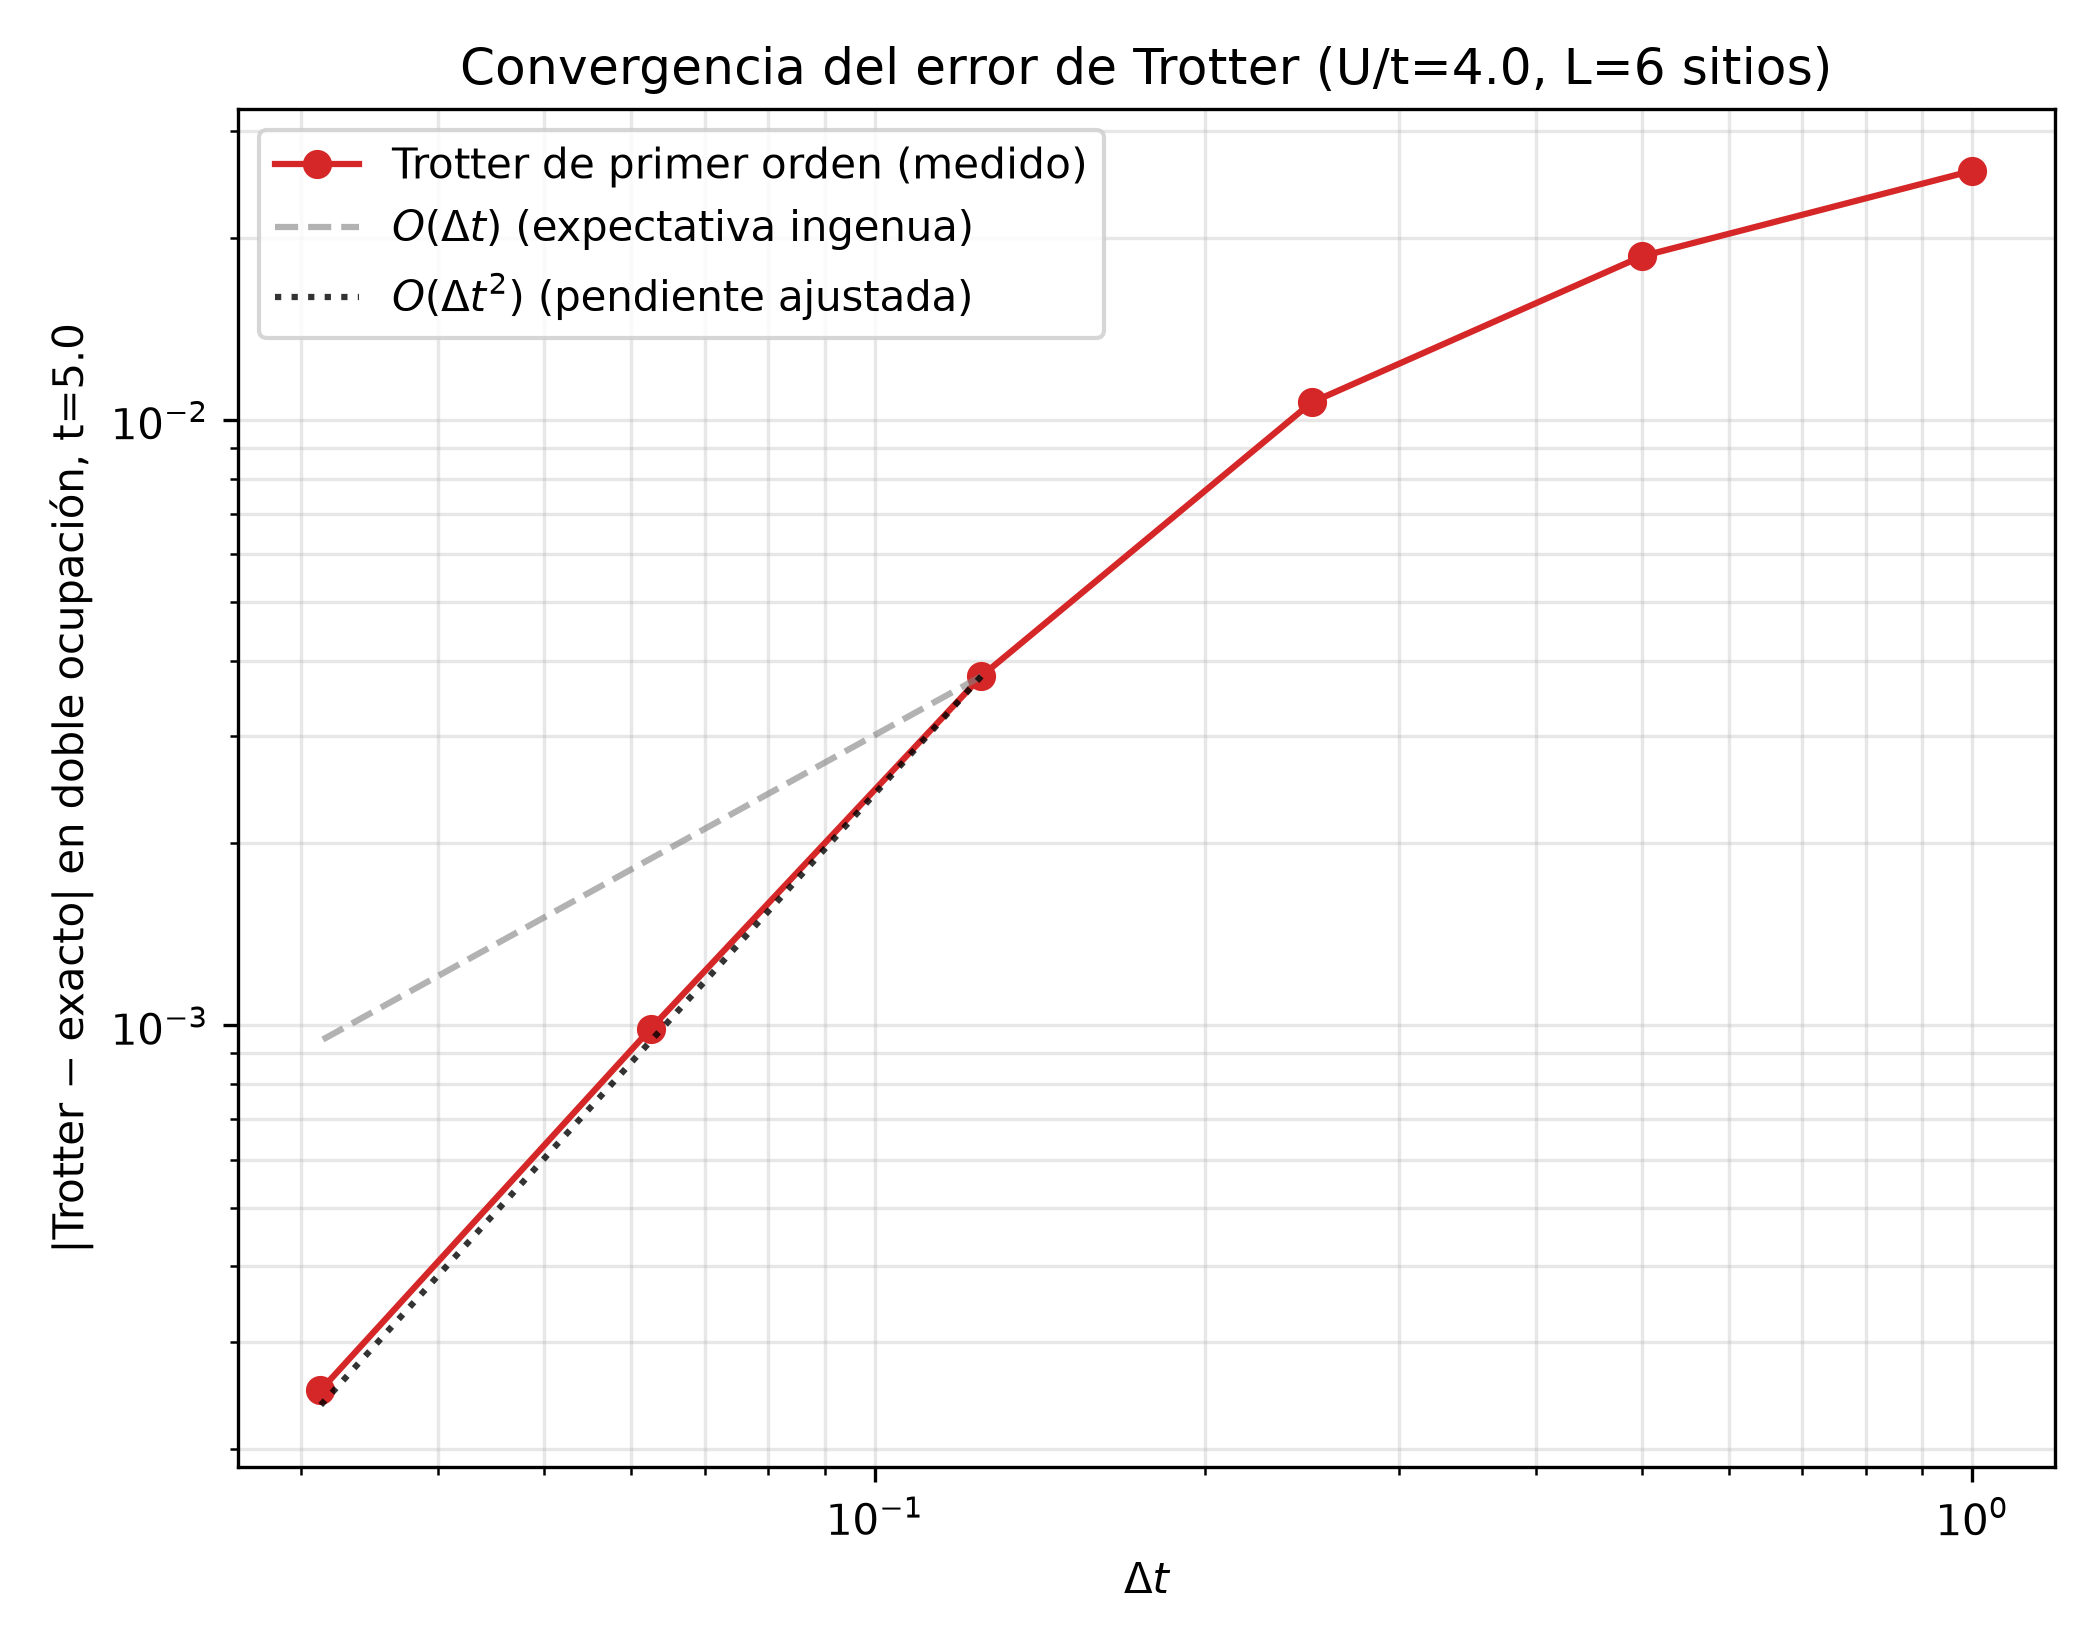
\includegraphics[width=\linewidth]{../fermi_hubbard_trotter_error_convergence.png}

    \clave{Pendiente 1.96 (1.98 en $4\times2$): más rápido que $O(\Delta t)$.}
  \end{block}
\end{column}

\begin{column}{0.02\paperwidth}\end{column}

\begin{column}{0.64\paperwidth}
  \begin{block}{5 · VQE (ansatz Hamiltoniano-Variacional, 48 parámetros)}
    \centering
    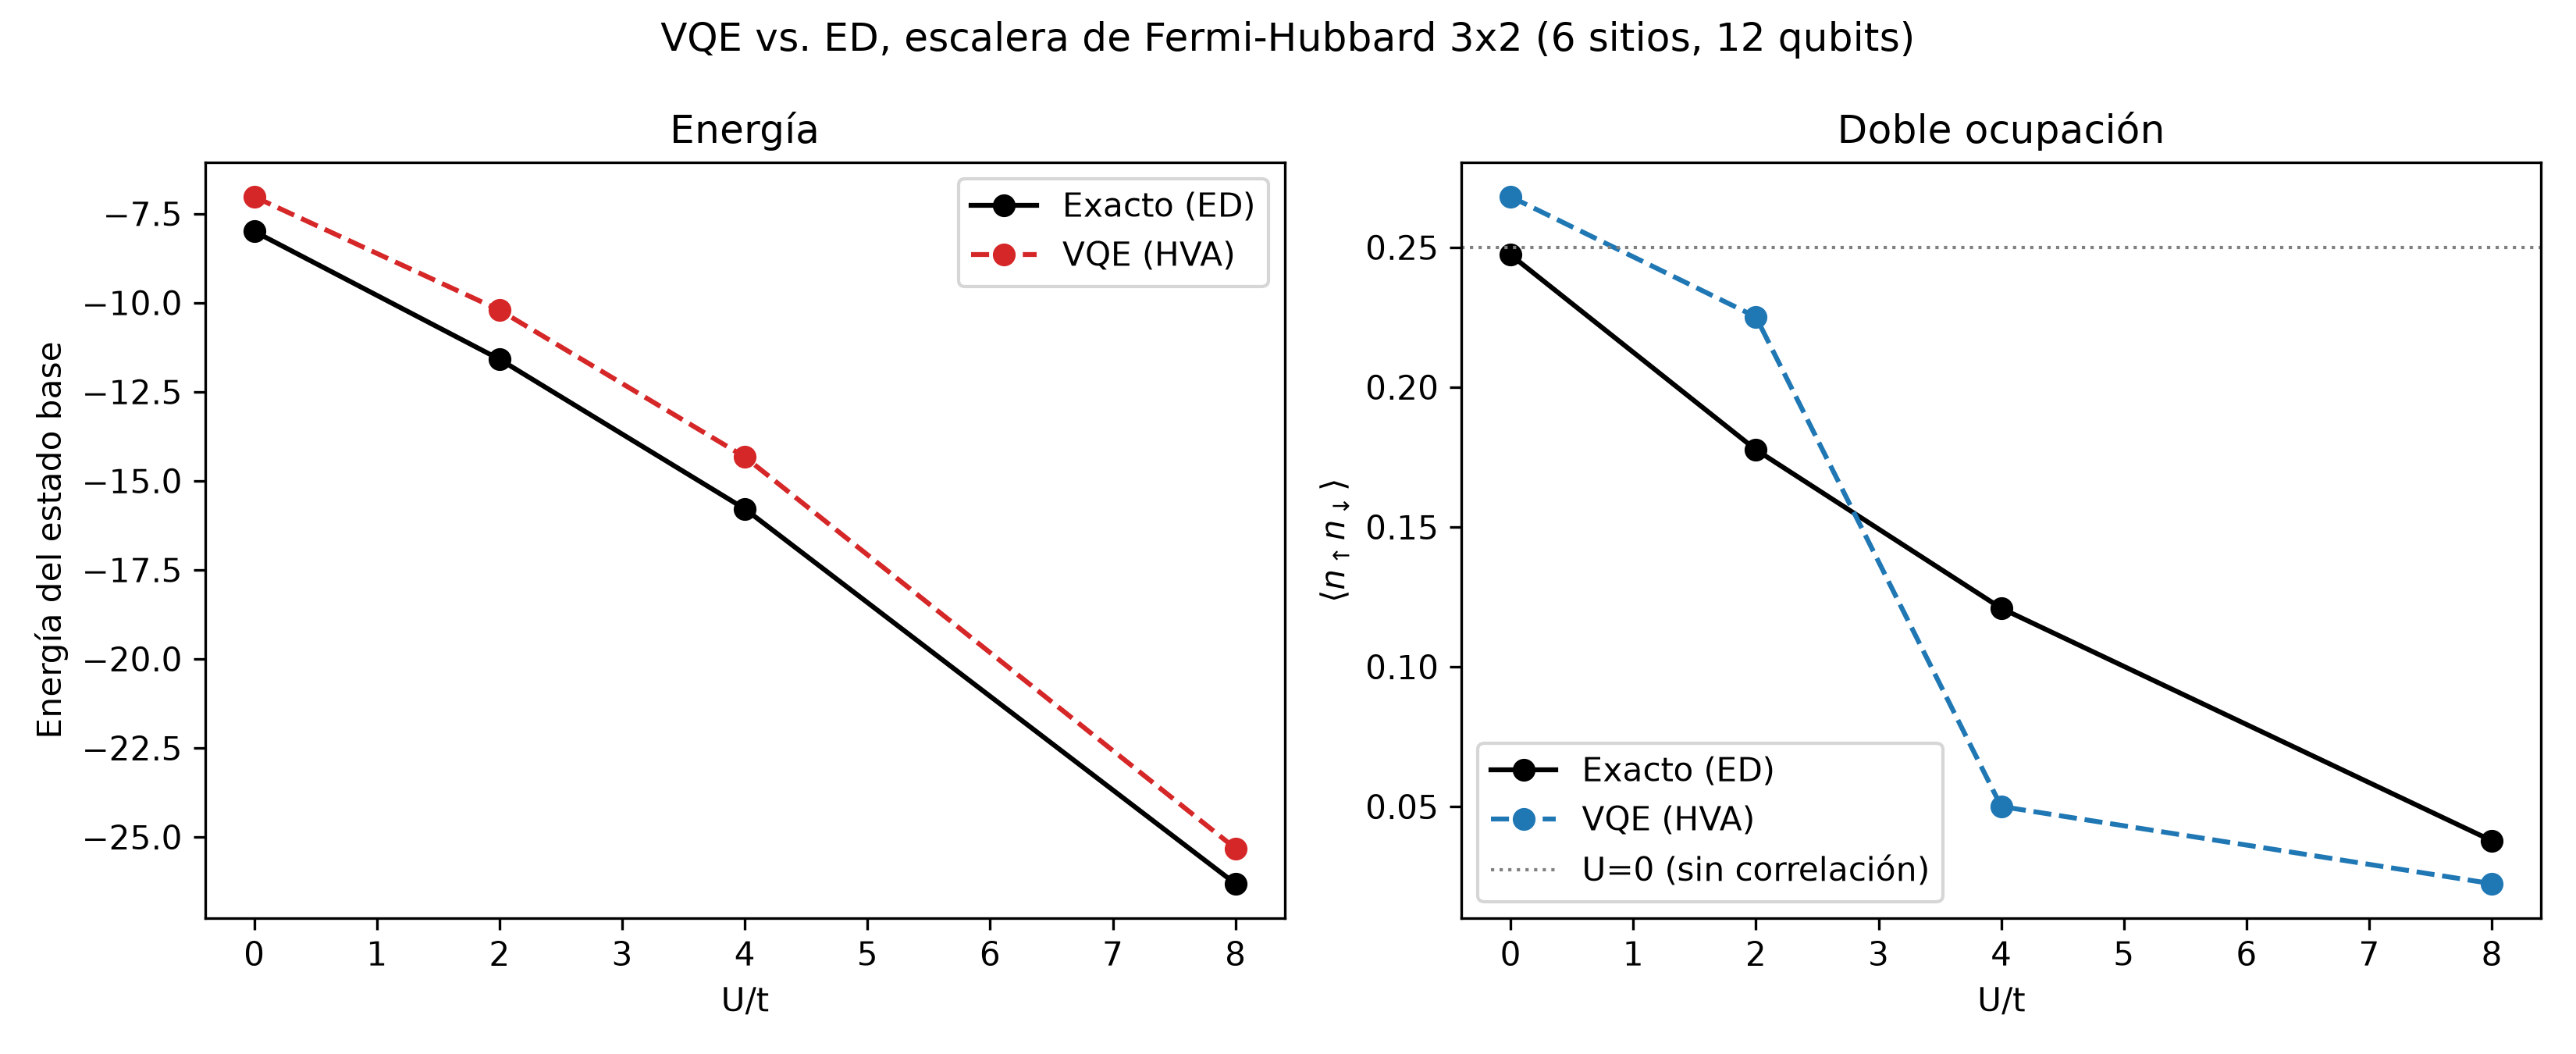
\includegraphics[width=\linewidth]{../fermi_hubbard_vqe_vs_ed.png}

    \clave{Tendencia correcta, pero $E$ queda 4--12\,\% arriba del exacto.}
  \end{block}
\end{column}

\begin{column}{0.02\paperwidth}\end{column}
\end{columns}

% =========================== FILA 4: CONCLUSIONES =========================
\vfill
\begin{columns}[T]
\begin{column}{0.02\paperwidth}\end{column}
\begin{column}{0.96\paperwidth}
  \begin{exampleblock}{Conclusiones}
    \begin{columns}[T]
      \begin{column}{0.49\linewidth}
        \begin{itemize}
          \item \good{Trotter reproduce la dinámica exacta.}
          \item \good{Su error es pequeño y medible} (pendiente $\approx2$).
        \end{itemize}
      \end{column}
      \begin{column}{0.49\linewidth}
        \begin{itemize}
          \item \warn{VQE es el cuello de botella} y fijó el tamaño del sistema.
          \item \warn{A 6 sitios domina el tamaño finito} (triplete hasta $U/t\approx4.3$).
        \end{itemize}
      \end{column}
    \end{columns}
  \end{exampleblock}
\end{column}
\begin{column}{0.02\paperwidth}\end{column}
\end{columns}

\end{frame}
\end{document}
